% Atualizado para atender as normas ABNT por Mônica da Silva (04/11/2021)

% --- -----------------------------------------------------------------
% --- Elementos usados na Capa e na Folha de Rosto.
% --- EXPRESSÔES ENTRE <> DEVERÂO SER COMPLETADAS COM A INFORMAÇÂO ESPECÍFICA DO TRABALHO
% --- E OS SÌMBOLOS <> DEVEM SER RETIRADOS 
% --- -----------------------------------------------------------------
\autor{PAULO CEZAR LACERDA NETO} % deve ser escrito em maiúsculo

\titulo{Aprendizado Profundo combinando Redes Convolucionais com Redes Recorrentes e Transformers para Apoio ao Diagnóstico da COVID-19 baseado em Tomografia Computacional de Tórax}

\instituicao{UNIVERSIDADE FEDERAL FLUMINENSE}

\orientador{CÉLIO VINICIUS NEVES DE ALBUQUERQUE}

\coorientadora{AURA CONCI} % se nao existir co-orientador apague essa linha

\local{NITER\'{O}I}

\data{2022} % ano da defesa

\comentario{Proposta de Tese de Doutorado apresentada ao Programa de P\'{o}s-Gradua\c{c}\~{a}o em Computa\c{c}\~{a}o da \mbox{Universidade} Federal Fluminense como requisito parcial para a obten\c{c}\~{a}o do Grau de \mbox{Doutor em Computa\c{c}\~{a}o}. \'{A}rea de concentra\c{c}\~{a}o: \mbox{Vis\~{a}o Computacional}} %preencha com a sua área de concentração


% --- -----------------------------------------------------------------
% --- Capa. (Capa externa, aquela com as letrinhas douradas)(Obrigatório)
% --- ----------------------------------------------------------------
\capa

% --- -----------------------------------------------------------------
% --- Folha de rosto. (Obrigatório)
% --- ----------------------------------------------------------------
\folhaderosto

% --- -----------------------------------------------------------------
% --- Ficha catalográfica obrigatória na versão final. (Obrigatório)
% --- ----------------------------------------------------------------

% \begin{figure}[!ht]
%   \centering
%   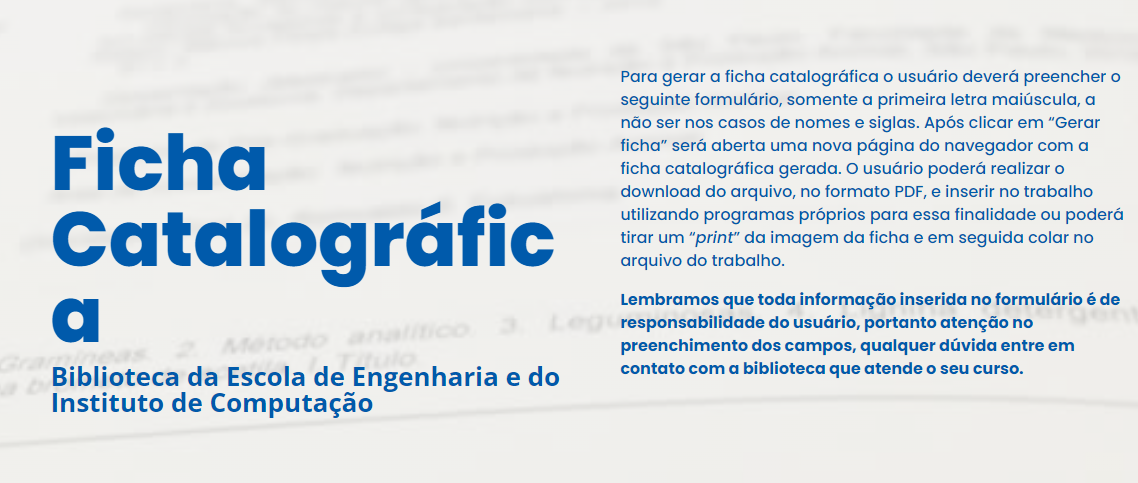
\includegraphics[width=1\linewidth]{capitulos/figuras/ficha_catalografica.png}
%   \caption{Ficha catalográfica}
% \end{figure}

% \cleardoublepage


% \pagestyle{ruledheader}
% \setcounter{page}{1}
% \pagenumbering{roman}

% --- -----------------------------------------------------------------
% --- Termo de aprovação. (Obrigatório)
% --- ----------------------------------------------------------------
\cleardoublepage
\thispagestyle{empty}

\vspace{-60mm}

\begin{center}
   {\large PAULO CEZAR LACERDA NETO}\\
   \vspace{7mm}

   APRENDIZADO PROFUNDO COMBINANDO REDES CONVOLUCIONAIS COM REDES RECORRENTES E TRANSFORMERS PARA APOIO AO DIAGNÓSTICO DA COVID-19 BASEADO EM TOMOGRAFIA COMPUTACIONAL DE TÓRAX\\
  \vspace{10mm}
\end{center}

\noindent
\begin{flushright}
\begin{minipage}[t]{10cm}
Proposta de Tese de Doutorado apresentada ao Programa de P\'{o}s-Gradua\c{c}\~{a}o em Computa\c{c}\~{a}o da Universidade Federal Fluminense como requisito parcial para a obten\c{c}\~{a}o do \mbox{Grau} de Doutor em Computa\c{c}\~{a}o. \'{A}rea de concentra\c{c}\~{a}o: \mbox{VIS\~{A}O COMPUTACIONAL} %preencha com a sua área de concentração

\end{minipage}
\end{flushright}
\vspace{0.5 cm}
\noindent
Maio de 2022. \\
\begin{flushright}
 % \parbox{11cm}
  {
  \begin{center}
  BANCA EXAMINADORA \\
  \vspace{5mm}
  \rule{11cm}{.1mm} \\
    Prof. Célio Vinicius Neves de Albuquerque - Orientador, UFF \\
    \vspace{3mm}
  \rule{11cm}{.1mm} \\
    Prof. Aura Conci, Co-orientadora, UFF\\
    \vspace{3mm}
  \rule{11cm}{.1mm} \\
    Prof. Anselmo Cardoso de Paiva, UFMA\\
  \vspace{3mm}
  \rule{11cm}{.1mm} \\
    Prof. Aristófanes Corrêa Silva, UFMA\\
    \vspace{3mm}
  \rule{11cm}{.1mm} \\
    Profa. Aline Marins Paes Carvalho, UFF\\
  \vspace{3mm}
  \end{center}
  }
\end{flushright}
\begin{center}
  \vspace{3mm}
  Niter\'{o}i \\
  2022

\end{center}

% --- -----------------------------------------------------------------
% --- Dedicatoria.(Opcional)
% --- -----------------------------------------------------------------
\cleardoublepage
\thispagestyle{empty}
\vspace*{200mm}

\begin{flushright}
{\em 
    Dedico esse trabalho a minha família por todo o seu apoio.
}
\end{flushright}
\newpage


% --- -----------------------------------------------------------------
% --- Agradecimentos.(Opcional)
% --- -----------------------------------------------------------------
\pretextualchapter{Agradecimentos}
\hspace{5mm}
Ao meu orientador e minha orientadora, que me mostraram os caminhos a serem seguidos e pela confiança depositada.



% --- -----------------------------------------------------------------
% --- Resumo em português.(Obrigatório)
% --- -----------------------------------------------------------------
\begin{resumo}


A pandemia da COVID-19 ocasionou milhões de casos da doença por todo o mundo, causada pelo coronavírus denominado SARS-CoV-2, gerando uma situação de emergência de saúde pública de âmbito mundial. 

Este trabalho propõe o desenvolvimento de um novo método para apoiar o diagnóstico de COVID-19, utilizando técnicas de processamento de imagens e aprendizado profundo aplicadas na análise de imagens médicas, mais especificamente imagens de tomografia computadorizada de tórax. A ideia é que o método possa ser utilizado por radiologistas para apoiar um diagnóstico rápido e eficaz da doença, reduzindo o impacto da COVID-19 e de outras doenças pulmonares no sistema de saúde. A metodologia do trabalho se baseia na construção de modelos  de aprendizado profundo, através da utilização de bases de dados públicas para treinamento de redes neurais convolucionais, em conjunto com técnicas de processamento de imagens, redes neurais recorrentes ou redes \textit{transformers} para a tarefa de classificação de imagens. O resultado esperado é que a abordagem proposta seja capaz de realizar as inferências em tempo real, com baixo custo e com resultados melhores do que outros métodos de última geração, em pelo menos uma das seguintes métricas: Sensibilidade, Especificidade, F1 Score e Área sob a Curva ROC.

{\hspace{-8mm} \bf{Palavras-chave}}: COVID-19; Aprendizado Profundo; Redes neurais convolucionais; Redes neurais recorrentes; Transformers; Diagnóstico auxiliado por computador

\end{resumo}

% --- -----------------------------------------------------------------
% --- Resumo em língua estrangeira.(Obrigatório)
% --- -----------------------------------------------------------------
\begin{abstract}

The COVID-19 pandemic caused by a virus called SARS-CoV-2, yielded millions of cases, provoking a public health emergency of international dimensions.

This work addresses the development of a method for analyzing medical images using image processing and deep learning techniques. The work methodology is based on the building of deep learning models, through the use of public databases for training convolutional neural networks, together with image processing techniques, recurrent neural networks, or \textit{transformers} networks for the classification task. The expected result is the proposed approach capable of making inferences in real-time, with the best results of other state-of-the-art methods, in at least one of the following measures: Sensitivity, Specificity, F1 Score, and Area under a ROC Curve.



{\hspace{-8mm} \bf{Keywords}}: COVID-19; Deep Learning; Convolutional neural networks; Recurrent neural networks; Transformers; Computer aided diagnostics.

\end{abstract}

% --- -----------------------------------------------------------------
% --- Lista de figuras.(Opcional)
% --- -----------------------------------------------------------------
%\cleardoublepage
\listoffigures



% --- -----------------------------------------------------------------
% --- Lista de tabelas.(Opcional)
% --- -----------------------------------------------------------------
\cleardoublepage
%\label{pag:last_page_introduction}
\listoftables
\cleardoublepage

% --- -----------------------------------------------------------------
% --- Lista de abreviatura.(Opcional)
%Elemento opcional, que consiste na relação alfabética das abreviaturas e siglas utilizadas no texto, seguidas das %palavras ou expressões correspondentes grafadas por extenso. Recomenda-se a elaboração de lista própria para cada %tipo (ABNT, 2005).
% --- ----------------------------------------------------------------

\cleardoublepage
% \printglossary[type=\acronymtype,title={Lista de Abreviaturas e Siglas}]
\pretextualchapter{Lista de Abreviaturas e Siglas}
\begin{tabular}{lcl}
AUC & : & \textit{Area Under ROC Curve};\\
CAD & : & \textit{Computer-Aided Diagnosis};\\
CNN & : & \textit{Convolutional Neural Network};\\
COVID-19 & : & \textit{Coronavirus Disease 2019};\\
GAP  & : & \textit{Global Average Pooling};\\
HPO & : & \textit{Hyperparemeter Optimization};\\
LSTM & : & \textit{Long Short-term Memory};\\
NIAB & : & \textit{Non-stochastic Infinite-armed Bandit};\\
PMC & : & Perceptron Multicamadas;\\
ReLU & : & \textit{Rectified Linear Activation Unit};\\
RNN & : & \textit{Recurrent Neural Network};\\
ROC & : & \textit{Receiver Operating Caracteristic};\\
RT-PCR & : & \textit{Reverse-Transcription Polymerase Chain Reaction};\\
SARS-Cov2 & : & \textit{Severe Acute Respiratory Syndrome Coronavirus 2};\\
TC & : & Tomografia Computadorizada;\\

\end{tabular}
\cleardoublepage


% --- -----------------------------------------------------------------
% --- Sumario.(Obrigatório)
% --- -----------------------------------------------------------------

\pagestyle{ruledheader}
\tableofcontents
\pagebreak